\chapter{Measurement}

\paragraph{Measurement} the process of empirical objective
assignment of values to entities,
in order to characterize a specific
attribute thereof.

\section{Measurement key element}

\begin{itemize}
  \item \textbf{Entity:} an object (either physical or virtual) or an event
  \item \textbf{Attribute:} a feature or property of an entity that is described or
        characterized
  \item \textbf{Objective:}  the process must be based on well-defined rules enabling
        repeatable results
\end{itemize}


\subsection{Construct vs. Indicator vs. Measure}


\begin{itemize}
  \item \textbf{Construct (Conceptual idea)}:
        Broad concept or topic of study. Abstract and possibly ambiguous. Not
        (always) directly observable. May be complex (multiple facets)

  \item \textbf{Indicator (Observable trait)}:
        Concrete, not ambiguous. Refer to a decision/interpretation model. Single
        facet

  \item \textbf{Measure (Operational definition)}: Precise definition. Clear measurement procedure
\end{itemize}


\begin{center}
  \begin{minipage}{0.75\linewidth}
    \begin{minipage}{0.47\linewidth}
      \centering
      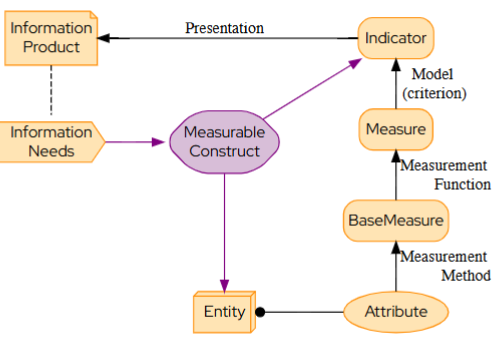
\includegraphics[width=\linewidth]{content/chapters/images/2026-05-26-20-23-06.png}
    \end{minipage}%
    \hfill
    \begin{minipage}{0.47\linewidth}
      \centering
      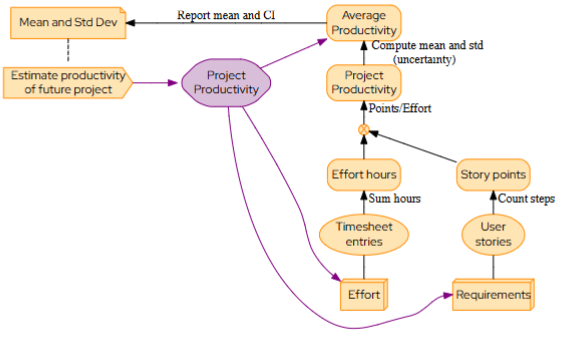
\includegraphics[width=\linewidth]{content/chapters/images/2026-05-26-20-23-29.png}
    \end{minipage}
  \end{minipage}
\end{center}

\subsection{Information needs}

The planning is driven by information needs dictated by
other processes. No (meaningful) measurement is possible without a clear
goa

\paragraph{Example of measures}

\begin{table}[h!]
  \renewcommand{\arraystretch}{1.4}
  \centering
  \begin{tabular}{lll}
    \toprule
    \multicolumn{1}{l}{\textbf{Entity}} & \multicolumn{1}{l}{\textbf{Attribute}} & \multicolumn{1}{l}{\textbf{Measure}} \\
    \midrule
    Person                              & Age                                    & Year of birthday                     \\
    Person                              & Age                                    & Months since birth                   \\
    Source code                         & Length                                 & \# Lines of Code (LOC)               \\
    Source code                         & Length                                 & \# Executable statements             \\
    Tester                              & Efficiency                             & \# of faults found / kLOC            \\
    Testing process                     & Fault frequency                        & \# of faults found / kLOC            \\
    Source code                         & Quality                                & \# of faults found / kLOC            \\
    \bottomrule
  \end{tabular}
\end{table}



\section{Types of measures}

\paragraph{Base measure}: Collected directly by interacting with the entity under
measurement. E.g.  elapsed time in hours, LOC, counting defects
\paragraph{Derived Measure}: Computed on the basis of other measures (either direct or
indirect). E.g. LOC/effort, \# defects/size, etc.




\begin{flushleft}
  \begin{minipage}[t]{0.45\linewidth}
    \raggedright
    \subsection{Internal}

    Internal measures can be measured purely in terms of the
    entity itself. e.g. length of source code (product)

  \end{minipage}%
  \hfill
  \begin{minipage}[t]{0.45\linewidth}
    \raggedright

    \subsection{External}

    External measures can only be measured with respect to
    how the entity relates to its environment. e.g. reliability of application (product)

  \end{minipage}
\end{flushleft}

Some attributes allow both internal and external measures,
e.g. Usability: Internal -> conformance to web standard;
External -> time to complete task

\begin{flushleft}
  \begin{minipage}[t]{0.45\linewidth}
    \raggedright
    \subsection{Objective}

    Objective measures do not depend on the environment or
    the person collecting the measure. Once you account for measurement error

  \end{minipage}%
  \hfill
  \begin{minipage}[t]{0.45\linewidth}
    \raggedright

    \subsection{Subjective}

    Subjective measures depend on the context where they are
    collected. Can change according to the person. They reflect the perception and judgment of the person
    performing the measurement
  \end{minipage}
\end{flushleft}


\begin{figure}[h!]
  \centering
  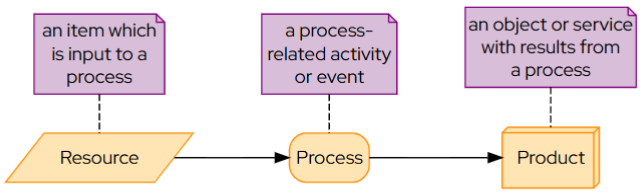
\includegraphics[width=0.4\linewidth]{content/chapters/images/2026-05-26-20-33-18.png}
\end{figure}

\section{Measurement Theory}

Scientific basis to determine formally:
\begin{itemize}
  \item What is an actual measure definition
  \item Which statements involving measures are meaningful
  \item What the appropriate scale type is
  \item What types of statistical operations can be applied to
        measurement data
\end{itemize}


\textbf{Representation problem:} The set of axioms under which measurement is possible.
Prescriptive theory: conditions for measurement

\textbf{Uniqueness problem:} How unique is the measure or scale.
Descriptive theory procedure, properties, scales

\subsection{Representational measurement}

The assignment of values must preserve any intuitive and
empirical observations about the attributes and entities
being measured.

Entities' attributes make sense only in terms of their relation to each other, e.
g., Joe is taller than Fred for people's height.
Therefore the same applies to the corresponding measures, e.g. 180cm > 172cm


\subsection{Empirical relation system}

A set of entities with their attributes, e.g., attribute height of entities people


The relations which are observed on entities in the ``real world'' which
characterize our understanding of the attribute in question, e.g., `Fred taller
than Joe'


The closed operations that can be performed on the objects, e.g.
put a person on the shoulder of another one

% ============================================================
% ! CONTINUA DA: Empirical relation system (fine del file .tex esistente)
% Inizia da slide 24 del PDF (pagina 25)
% ============================================================

\subsection{Measurement Mapping}

Mapping from the empirical relation system onto a formal relation system. Consists of:
\begin{itemize}
  \item Metric
  \item Relation mapping
\end{itemize}

A.k.a. representation, homomorphism.

\paragraph{Measure} the value (formal element) assigned to an entity in order to characterize an attribute.

% [Immagine: slide 25 - Measurement mapping diagram:
%  riquadro "Empirical system" (Joe is taller than Fred) → mapping →
%  riquadro "Formal system" (M(Joe)=180, M(Fred)=172, M(Joe)>M(Fred))]

\subsection{Representation Condition}

The measurement mapping implies that all empirical relations are preserved in formal
(numerical) relations and no new relation is introduced
(e.g.\ $M(\text{Fred}) > M(\text{Joe})$ precisely when Fred is taller than Joe).

A metric is called \textbf{admissible} if the representation condition holds (measurement scale).

\subsection{Formal Definition}

A homomorphism $m$ from the empirical system to the formal system.
\begin{itemize}
  \item \textbf{scale:} $(\mathfrak{E},\mathfrak{F},m)$
  \item \textbf{empirical system:} $\mathfrak{E}=(E,\text{taller})$
  \item \textbf{formal system:} $\mathfrak{F}=(\mathbb{R},>)$
  \item \textbf{mapping function:} $m:E\rightarrow\mathbb{R} \mid \forall a,b\in E: a \text{ taller } b \Rightarrow m(a)>m(b)$
\end{itemize}

\subsection{Extensive Metric}

The empirical system also defines a concatenation operation.
\begin{itemize}
  \item \textbf{scale:} $(\mathfrak{E},\mathfrak{F},m)$
  \item \textbf{empirical system:} $\mathfrak{E} = (E, \text{taller}, \text{piled})$
  \item \textbf{formal system:} $\mathfrak{F}=(\mathbb{R},>,+)$
  \item \textbf{mapping function:} $m:E\rightarrow\mathbb{R} \mid \forall a,b\in E: a \text{ taller } b \Rightarrow m(a)>m(b) \wedge m(a \text{ piled } b)=m(a)+m(b)$
\end{itemize}

\subsection{Admissible Transformation}

Metrics are not unique: in general there are several homomorphisms that satisfy the
representation condition. An \textbf{admissible transformation} $\Phi$:
\begin{itemize}
  \item $\Phi \circ m$ is a homomorphism
  \item Mapping between two measures, e.g.\ length:
        \begin{itemize}
          \item Admissible transformation: $M' = a \cdot M$
          \item Inadmissible transformation: $M' = a \cdot M + b$
        \end{itemize}
\end{itemize}

\subsection{Relation System Richness}

$RS_A$ is richer than $RS_B$ if all relations in $RS_B$ are contained in $RS_A$.
The richer the empirical system, the more sophisticated the scale.
Complex and well-understood phenomena require more sophisticated measurement scales.

\begin{itemize}
  \item \textbf{``Poor'' Relation System}: only equivalence (same/different). Example: food
        category (fruit, root, mushroom)
  \item \textbf{``Less poor'' Relation System}: ordering relation (higher/lower). Example:
        place of growth w.r.t.\ ground (above/on/below ground)
  \item \textbf{``Rich'' Relation System}: ordering + concatenation ($<$, $+$). Example:
        protein content per 100g
\end{itemize}

% ============================================================
\section{Measurement Scales}
% ============================================================

\subsection{Scale Classification}

Measurement scales can be classified according to the class of admissible transformations:
\begin{itemize}
  \item The \textbf{larger} the set of admissible transformations $\Rightarrow$ the looser,
        less accurate, and less rich the scale
  \item The \textbf{smaller} the set of admissible transformations $\Rightarrow$ the more
        accurate and richer the scale
\end{itemize}

Scale types: \textbf{Nominal}, \textbf{Ordinal}, \textbf{Interval}, \textbf{Ratio}, \textbf{Absolute}.

\subsection{Binary Nominal Scale}

Places elements in a classification scheme; similar examples are part of the same class.
Empirical relation: different classes — no ordering relation.
Any distinct numbering or symbolic representation is acceptable; no notion of magnitude.

Equivalence relation $\sim$ (symmetric, reflexive, transitive):

\begin{itemize}
  \item \textbf{scale:} $(\mathfrak{E},\mathfrak{F},m)$
  \item \textbf{empirical system:} $\mathfrak{E}=(E,\sim)$
  \item \textbf{formal system:} $\mathfrak{F}=(\mathbb{R},=)$
  \item \textbf{mapping function:} $m:E\rightarrow\mathbb{R} \mid \forall a,b\in E:a\sim b\iff m(a)=m(b)$
\end{itemize}

\paragraph{Examples}
\begin{itemize}
  \item Entity: person; Attribute: origin (Italy / EU / Extra-EU):
        $M(p) = 1$ if from Italy, $2$ if from any EU country, $3$ if from a non-EU country
  \item Entity: fault; Attribute: location (Specification / Design / Code):
        $M(x) = 1$ if specification fault, $2$ if design fault, $3$ if code fault
\end{itemize}

\paragraph{Nominal Statistics}
Only base operation: \textbf{count}. Available statistics: frequency (per category), mode.

\subsection{Ordinal Scale}

Empirical system: classes of entities ordered w.r.t.\ attribute. Empirical relation: total order.
Acceptable mapping: any mapping preserving the order. Measure represents ranking only.
\begin{itemize}
  \item Acceptable transformations: all monotonic increasing mappings
  \item $\langle C_1, C_2, \ldots, C_n \rangle \to \langle a_1, a_2, \ldots, a_n \rangle$
        where $\forall i, j : i > j \Rightarrow a_i > a_j$
\end{itemize}

\subsection{Binary Ordinal system}


Weak order relation $\succ$ (reflexive, transitive):

\begin{itemize}
  \item \textbf{scale:} $(\mathfrak{E},\mathfrak{F},m)$
  \item \textbf{empirical system:} $\mathfrak{E}=(E,>)$
  \item \textbf{formal system:} $\mathfrak{F}=(\mathbb{R},\ge)$
  \item \textbf{mapping function:} $m:E\rightarrow\mathbb{R} \mid \forall a,b\in E:a>b\iff m(a)\ge m(b)$
\end{itemize}

\paragraph{Example}
Entity: person; Attribute: agreement with statement.
$\text{Completely disagree} \prec \text{Partly disagree} \prec \text{Partly agree} \prec \text{Completely agree}$



\vspace{1cm}
Admissible mapping: $M(x) = 1, 2, 3, 4$ respectively for Completely disagree to Completely agree.

\subsection{Ordinal Statistics}

\paragraph{Operations:} counting, sorting.
\paragraph{Available statistics:} frequency (per category), mode, rank,
quantiles (median).

\subsection{Interval Scale}

Empirical system: order and differences between classes.
Empirical relation: distance from a reference point.
Acceptable mappings preserve order and difference — addition and subtraction make sense,
but the ratio does not.
Admissible transformations: \textbf{affine transformations} $M' = a \cdot M + b$ (with $a > 0$).

Comparison of intervals $(a, b) \succsim (c, d)$ (reflexive, transitive).

\paragraph{Example}
Entity: activity; Attribute: start day.
\begin{itemize}
  \item Gregorian calendar: $D_G = 36$ (Feb 5, 2019)
  \item Chinese lunar calendar: $D_C = 1$ (1st day, 1st Month, Year of the Pig)
  \item Admissible transformation: $D_G = D_C + 36$
\end{itemize}

\paragraph{Interval Statistics}
Operations: counting, sorting, sum, difference, scalar division.
Available statistics: frequency, mode, rank, quantiles, mean (arithmetic average), variance
(and derivatives).

\subsection{Ratio Scale}

Empirical system: there is a zero element representing total lack of attribute.
Measurement starts at zero and increases at equal intervals (units).
Empirical relation: ratio between entities.
Admissible transformations: $M' = a \cdot M$ (with $a > 0$).

\paragraph{Extensive System}
Concatenation operation $\circ$:
\begin{itemize}
  \item Associative
  \item Monotone
  \item Archimedean postulate: $p \succ r \Rightarrow \exists\, n \in \mathbb{N} \mid n \cdot r \succ p$
        (where $n \cdot r = r \circ r \circ \ldots \circ r$ for $n$ times)
\end{itemize}

\paragraph{Example}
Entity: person; Attribute: age.
Admissible transformation: $M_{\text{months}} = 12 \cdot M_{\text{year}}$.

\subsection{Ratio Statistics}
\textbf{Operations:} counting, sorting, sum, difference, scalar division, division, (multiplication).

\textbf{Available statistics:} all interval statistics + standardized mean difference, geometric mean, etc.

\subsection{Absolute Scale}

Measurement made by counting items in the entity set:
\begin{itemize}
  \item Number of occurrences
  \item Only one possible mapping
  \item All arithmetic analysis is meaningful
\end{itemize}

Empirical system: Entity (project) and Attribute (full time staff).
Number of full time developers.

The attribute definition implies the items to be counted. Length is \emph{not} measurable on an
absolute scale (\# of lines is); age is \emph{not} measurable on an absolute scale.

\subsection{Scales Summary}

\begin{table}[h!]
  \renewcommand{\arraystretch}{1.4}
  \centering
  \begin{tabular}{lll}
    \toprule
    \textbf{Scale} & \textbf{Admissible Transformations} & \textbf{Example}           \\
    \midrule
    Nominal        & 1-to-1 mapping                      & Labeling, classifying      \\
    Ordinal        & Monotonic increasing function       & Preference, hardness       \\
    Interval       & $M' = a \cdot M + b$, $a > 0$       & Relative time, temperature \\
    Ratio          & $M' = a \cdot M$, $a > 0$           & Time interval, length      \\
    Absolute       & $M' = M$                            & Counting entities          \\
    \bottomrule
  \end{tabular}
\end{table}

% ============================================================
\section{Meaningful Statements and Operations}
% ============================================================

\paragraph{Meaningful statement}
A statement involving measurement is meaningful if its truth is invariant of transformation
to any admissible scale (i.e.\ the conclusion is the same after an admissible transformation
is applied to the measures).

\paragraph{Meaningful statements}

The cost of fixing each error is at least 100.
A semantic error is twice as complex as a syntactic error

\paragraph{Meaningful statements?}
\begin{itemize}
  \item ``Fred is twice as tall as Jane'' $\to$ \textbf{Yes}, truth invariant of any scale
  \item ``The temperature in Tokyo today is twice that in London'' $\to$ \textbf{No},
        truth depends on the scale (Celsius 18:9 vs.\ Fahrenheit 64:48)
  \item ``The difference in temperature between Tokyo and London today is twice what it was
        yesterday'' $\to$ \textbf{Yes}, ratios of differences are preserved by affine
        transformations
\end{itemize}

\paragraph{Meaningful operation}
An operation is meaningful if the conclusions are invariant of transformation to any
admissible scale.

\subsection{Statistical Operations — Central Tendency}

\begin{table}[h!]
  \renewcommand{\arraystretch}{1.4}
  \centering
  \begin{tabularx}{0.6\textwidth}{>{\raggedright\arraybackslash}X >{\centering\arraybackslash}X >{\centering\arraybackslash}X >{\centering\arraybackslash}X}
    \toprule
    \textbf{Type} & \textbf{Mean} & \textbf{Median} & \textbf{Mode} \\
    \midrule
    Nominal       & $-$           & $-$             & $+$           \\
    Ordinal       & $-$           & $+$             & $+$           \\
    Interval      & $+$           & $+$             & $+$           \\
    Ratio         & $+$           & $+$             & $+$           \\
    Absolute      & $+$           & $+$             & $+$           \\
    \bottomrule
  \end{tabularx}
\end{table}

% ============================================================
\section{Indicators}
% ============================================================

An indicator is defined by:
\begin{itemize}
  \item \textbf{Name}
  \item \textbf{Goal}
  \item \textbf{Metric definition}: how computed, unit of measure, scale, aggregation
  \item \textbf{Interpretation}
  \item \textbf{Source}: where the data comes from
\end{itemize}

\subsection{Interpretation}



\begin{flushleft}
  \begin{minipage}{0.65\linewidth}
    \raggedright
    Interpretation entails a reference. Typical references:
    \begin{itemize}
      \item \textbf{Conformance}: compare to a specific business or usage requirement
      \item \textbf{Benchmark}: compare with a benchmark for similar product or system
      \item \textbf{Time series}: observe trend in time
      \item \textbf{Population norms}: compute quantile — requires a DB of previous values
    \end{itemize}

  \end{minipage}%
  \hfill
  \begin{minipage}{0.3\linewidth}
    \centering
    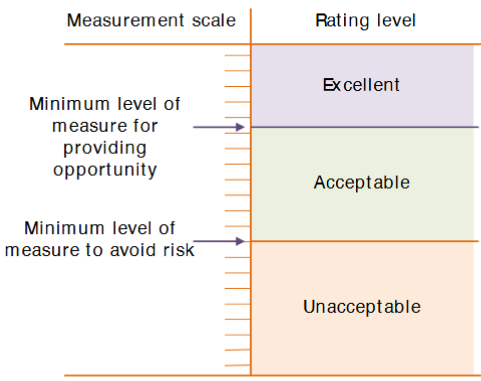
\includegraphics[width=\linewidth]{content/chapters/images/2026-05-26-21-23-45.png}
  \end{minipage}
\end{flushleft}





\begin{flushleft}
  \begin{minipage}[t]{0.45\linewidth}
    \raggedright
    \subsection{Indicator Robustness}

    \begin{itemize}
      \item \textbf{Comprehensibility / Understandability}: how simple
      \item \textbf{Processing Cost}: initial and incremental
      \item \textbf{Significance / Meaningfulness}: how much it covers the information need
      \item \textbf{Frequency}: how often indicator varies
      \item \textbf{Structuredness}: how much it is objective/not ambiguous
    \end{itemize}

  \end{minipage}%
  \hfill
  \begin{minipage}[t]{0.45\linewidth}
    \raggedright
    \subsection{SMART Indicators}

    \begin{itemize}
      \item \textbf{S}pecific in purpose
      \item \textbf{M}easurable
      \item \textbf{A}chievable
      \item \textbf{R}elevant
      \item \textbf{T}imely
    \end{itemize}

  \end{minipage}
\end{flushleft}


\subsection{Aggregation Dimensions Or segmentation}

Entities to which the indicator is associated and therefore data the indicator can be
aggregated on (also called segmentation). Dimensions are typically nominal or ordinal metrics.

A dimension is defined by a characteristic and an attribute. In practical terms they are
often nominal or ordinal measures not directly linked to the objective of the indicator.

\paragraph{Common dimensions}
\begin{itemize}
  \item \textbf{Time window}: e.g. sales per hour/day/month
  \item \textbf{Hierarchical node} in org./geo structure:
        e.g. sales per country/region/shop; expenses per company/division/group/person
  \item \textbf{Product/product category}: e.g. sales per phone xy / per business phones
  \item \textbf{Customer/customer category}: e.g. gender or sensitive features
  \item \textbf{Activity in process}: e.g. cost, defects for design or production
  \item \textbf{Project}: e.g. cost, defects per project
\end{itemize}

% ============================================================
\section{Measurement Process}
% ============================================================

% [Immagine: slide 79 - Measurement Process diagram (adattato da ISO/IEC 15939:2007)
%  Nodi: "Establish & sustain commitment" → "Plan" → "Perform" → "Evaluate"
%  con "Experience base" che alimenta Plan e Perform, e "Tech/Mgmt Process" in cima]




\begin{flushleft}
  \begin{minipage}{0.65\linewidth}
    \raggedright
    \paragraph{Measurement guiding principle}

    \begin{quote}
      \textit{What gets measured gets done.} \hfill (attributed to P.\ Drucker)
    \end{quote}

    \paragraph{Campbell's Law}

    \begin{quote}
      \textit{The more any quantitative social indicator is used for social decision-making,
        the more subject it will be to corruption pressures and the more apt it will be to distort
        and corrupt the social processes it is intended to monitor.}
      \hfill (Donald T.\ Campbell)
    \end{quote}

    \paragraph{Goodhart's Law}

    \begin{quote}
      \textit{When a measure becomes a target, it ceases to be a good measure.}
      \hfill (J.\ Goodhart)
    \end{quote}

  \end{minipage}%
  \hfill
  \begin{minipage}{0.3\linewidth}

    \centering
    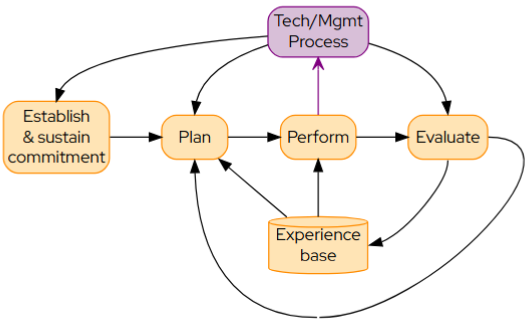
\includegraphics[width=\linewidth]{content/chapters/images/2026-05-26-21-30-08.png}

  \end{minipage}
\end{flushleft}


% ============================================================
\section{Software Base Measures}
% ============================================================

\subsection{Product Metrics — Internal Attributes}

\begin{itemize}
  \item Few simple and easy to measure (e.g.\ size)
  \item Others controversial (e.g.\ complexity)
  \item Automated measurement
\end{itemize}

Methodologies address structuring and improvement of software products in terms of
development process and products, typically characterized by internal attributes.
Quality assurance: internal attributes can be measured during development to predict
and control external ones.

\subsection{Process Measures}

\begin{itemize}
  \item \textbf{Duration}: of process or one of its activities
  \item \textbf{Effort}: in process or one of its activities
  \item \textbf{Number of events}: of a given type, arising during process or one of
        its activities
  \item \textbf{Subjective measures}
\end{itemize}

\subsection{Resource Measures}

Input for sw development process:

\begin{flushleft}
  \begin{minipage}[t]{0.45\linewidth}
    \raggedright
    \textbf{Resources}
    \begin{itemize}
      \item \textbf{Personnel}: individuals and teams
      \item \textbf{Materials}: e.g.\ office supplies
      \item \textbf{Tools}: both HW and SW
      \item \textbf{Methods}
    \end{itemize}
  \end{minipage}%
  \hfill
  \begin{minipage}[t]{0.45\linewidth}
    \raggedright
    \textbf{Resource metrics}
    \begin{itemize}
      \item \textbf{Magnitude}: e.g.\ how many staff?
      \item \textbf{Cost}: e.g.\ payments for testing tools
      \item \textbf{Quality}: e.g.\ experience of developers
    \end{itemize}
  \end{minipage}
\end{flushleft}

\[
  \text{Productivity} = \frac{\text{Amount of output}}{\text{Effort input}}
\]

\subsection{Quality Measure Elements (QME)}

% [Immagine: slide 91 - Quality Measure Elements mind map
%  Nodo centrale "Quality Measure Elements" con rami:
%  Time (User time, System operation time, Execution time, Time interval, Effort)
%  Size (Program size, Used resources, Functional size, Operating procedure steps)
%  Count (No. detected faults, No. changes, No. strokes, No. detected failures,
%         No. attempts, Structural Complexity, No. detected inconsistencies, Score)]


\begin{flushleft}
  \begin{minipage}[t]{0.45\linewidth}
    \raggedright
    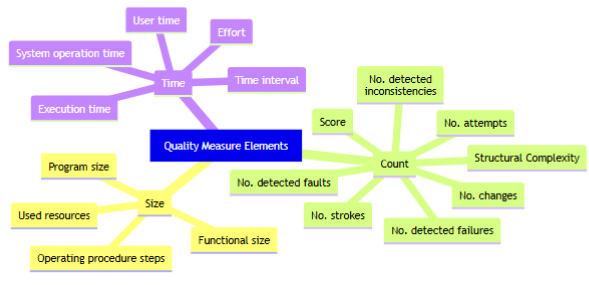
\includegraphics[width=\linewidth]{content/chapters/images/2026-05-26-21-31-43.png}
    \captionof{figure}{Quality Measure Elements}


  \end{minipage}%
  \hfill
  \begin{minipage}[t]{0.45\linewidth}
    \raggedright
    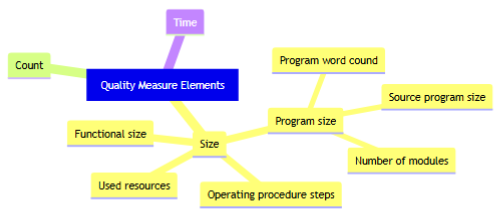
\includegraphics[width=\linewidth]{content/chapters/images/2026-05-26-21-31-57.png}
    \captionof{figure}{QMEs: size}


  \end{minipage}
\end{flushleft}


\subsubsection{QMEs: Size}

\begin{itemize}
  \item \textbf{Program size}: e.g.\ program word count, number of modules
  \item \textbf{Functional size}
  \item \textbf{Used resources}
  \item \textbf{Operating procedure steps}
\end{itemize}

\paragraph{Functional Size}
Function Point Analysis, developed by Allan J.\ Albrecht in the late 1970s.
Several ISO standards:
ISO/IEC 19761 (COSMIC method), ISO/IEC 20926 (IFPUG method), ISO/IEC 20968 (Mk II method),
ISO/IEC 24570 (NESMA method), ISO/IEC 29881 (FiSMA method). Also: Use Case Points.

\paragraph{COSMIC FP — Principles}
\begin{itemize}
  \item Software interacts with its users across a boundary, and with storage
  \item User requirements can be mapped into unique functional processes
  \item Each functional process consists of sub-processes: a data movement or a data
        manipulation
  \item A data movement moves a single data group:
        \begin{itemize}
          \item \textbf{Entry}: data from user to system
          \item \textbf{Exit}: data from system to user
          \item \textbf{Write}: data from system to persistent storage
          \item \textbf{Read}: data from persistent storage to system
        \end{itemize}
  \item \textbf{Data group}: set of attributes that describe a single object of interest
  \item Each process is started by its triggering Entry data movement
\end{itemize}

\paragraph{Use Case Points — Principles}
\begin{itemize}
  \item Actor types: Simple / Average / Complex $\to$ UAW
  \item Use case types: Simple / Average / Complex $\to$ UUCW
  \item Technical Complexity Factors: factor weight $\times$ influence $\to$ TCF
  \item Environmental Factors: factor weight $\times$ influence $\to$ EF
\end{itemize}
\[
  UCP = (UAW + UUCW) \times TCF \times EF
\]

\paragraph{Lines of Code (LOC)}
Most intuitive size measure — count the number of lines of code.
NCSS = Non-Comment Source Statements.

Operational aspects:
\begin{itemize}
  \item Multiple instructions on a line: number of statements vs.\ number of lines
  \item Inclusion/exclusion of: executable statements, data declarations, comments,
        compiler directives
\end{itemize}

\textbf{Pros \& Cons:}
\begin{itemize}
  \item[$+$] Easy to understand
  \item[$+$] Easy approximate measure (e.g.\ \texttt{wc -l *.c})
  \item[$+$] Very widely used; several predictive models use LOC
  \item[$-$] Hard to measure precisely
  \item[$-$] If used to measure productivity, does not favor well-structured programs
\end{itemize}



\begin{flushleft}
  \begin{minipage}{0.65\linewidth}
    \subsubsection{QMEs: Time}

    \raggedright

    \begin{itemize}
      \item \textbf{Real time unit}: physical time (second, minute, hour)
      \item \textbf{Computer machinery time unit}: CPU time
      \item \textbf{Official scheduled time unit}: working hours, calendar days, months or years
      \item \textbf{Component time unit}: accumulation of individual time of each site
      \item \textbf{System time unit}: considers all sites as a whole
    \end{itemize}

  \end{minipage}%
  \hfill
  \begin{minipage}{0.3\linewidth}

    \raggedright
    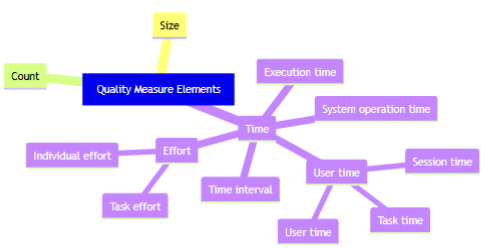
\includegraphics[width=\linewidth]{content/chapters/images/2026-05-26-21-34-04.png}
  \end{minipage}
\end{flushleft}


\paragraph{Effort}
\begin{itemize}
  \item \textbf{Individual effort}: productive time required for a person to complete his/her
        part of a task; fixed number of productive hours per day
  \item \textbf{Task effort}: accumulated value of all individual project personnel
        (developer, maintainer, operator, user, or others) who worked to complete a
        specified task
\end{itemize}




\begin{flushleft}
  \begin{minipage}{0.65\linewidth}
    \raggedright
    \subsubsection{QMEs: Count}

    \begin{itemize}
      \item No.\ attempts, no.\ changes, no.\ detected failures, no.\ strokes
      \item \textbf{Structural Complexity}
      \item No.\ detected inconsistencies, no.\ detected faults, score
    \end{itemize}
  \end{minipage}%
  \hfill
  \begin{minipage}{0.3\linewidth}
    \centering
    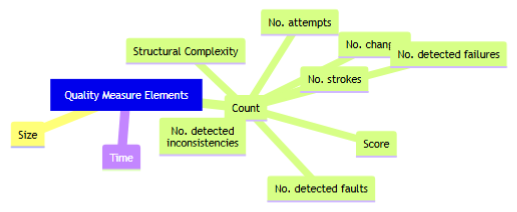
\includegraphics[width=\linewidth]{content/chapters/images/2026-05-26-21-35-15.png}
  \end{minipage}
\end{flushleft}


\subsection{McCabe Cyclomatic Complexity}

Measures complexity of the control flow.
Control flow is represented as a Control Flow Graph (CFG):
\begin{itemize}
  \item Nodes are statements
  \item Edges are possible sequences of statements
\end{itemize}

$V(G)$ is the number of base paths in $G$ — the number of linearly independent paths from
initial node to final node.

\paragraph{Cyclomatic number}
If $G$ is a strongly connected graph: $V(G) = \#E - \#N + 1$

A typical CFG is not strongly connected (unless we add an edge from the final to the
initial node):$V(G) = \#E - \#N + 2$

\begin{flushleft}
  \begin{minipage}{0.42\linewidth}
    \raggedright
    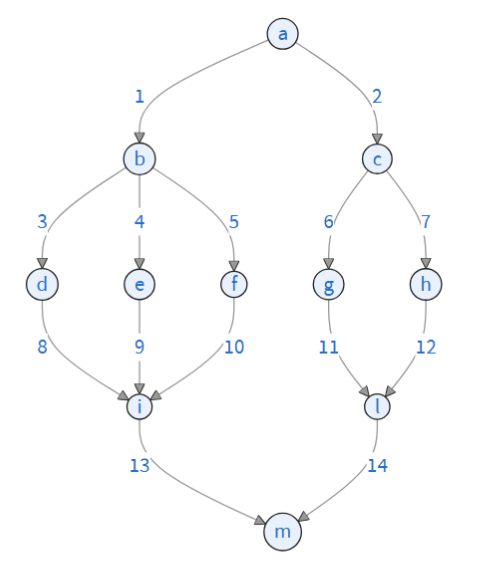
\includegraphics[width=0.6\linewidth]{content/chapters/images/2026-05-26-21-36-23.png}
  \end{minipage}%
  \hfill
  \begin{minipage}{0.52\linewidth}
    Paths in the example:
    \begin{itemize}
      \item C1: 1, 3, 8, 13
      \item C2: 1, 4, 9, 13
      \item C3: 1, 5, 10, 13
      \item C4: 2, 6, 11, 14
      \item C5: 2, 7, 12, 14
    \end{itemize}
    \[V(G) = E - N + 1 = 14 - 11 + 2 = 5\]
  \end{minipage}
\end{flushleft}

\paragraph{Cyclomatic complexity in practice}
Start at 1; iterate on all statements; add 1 for every complexity-incrementing statement.
For Java: \texttt{if, for, while, case, catch, throw, \&\&, ||, ?}

\paragraph{CC Thresholds} (much debated)
\begin{itemize}
  \item 1--10: Low risk routine
  \item 11--20: Moderate risk
  \item 21--50: High risk
  \item $> 50$: Most complex and highly unstable
\end{itemize}

\paragraph{McCabe Pros \& Cons}
\begin{itemize}
  \item[$+$] Well defined from a mathematical point of view
  \item[$+$] Typically strongly correlated with LOC
  \item[$+$] Focus on code complexity
  \item[$-$] Disregards data-related complexity
\end{itemize}

% [Immagine: slide 109 - CC vs.\ LoCs scatter plot
%  "Cyclomatic complexity v.\ executable lines" (da Les Hatton)
%  Asse X: Cyclomatic complexity (0--400), Asse Y: XLOC (0--1400)]

\subsection{Design Metrics — CK (Chidamber \& Kemerer)}

\begin{itemize}
  \item \textbf{WMC} (Weighted Methods per Class): count of methods in each class
  \item \textbf{NOC} (Number Of Children per class): number of immediate sub-classes of
        a class
  \item \textbf{DIT} (Depth of Inheritance Tree): maximum inheritance path from the class
        to the root class
  \item \textbf{CBO} (Coupling Between Object classes): number of classes to which a class
        is coupled
  \item \textbf{RFC} (Response For a Class): sum of cardinalities of methods in the class
        and remote methods directly called by methods of the class
  \item \textbf{LCOM} (Lack of Cohesion in Methods): where $Q$ = \# pairs of methods
        sharing attributes, $P$ = \# pairs of methods not sharing attributes
\end{itemize}

\paragraph{LCOM --- Henderson-Sellers (alternative definition)}

\[
  LCOM_2 = 1 - \frac{\sum m_{A_i}}{m \cdot a}
\]

\vspace{0.5cm}
where $m$ = number of methods in class, $a$ = number of attributes in class,
$m_{A_i}$ = number of methods using attribute $A_i$.

\paragraph{CK Pros \& Cons}
\begin{itemize}
  \item[$-$] Theoretical validation lacking
  \item[$-$] Empirical validation lacking
  \item[$-$] Not all metrics can be easily computed: RFC and LCOM need implementation
        details (design or code metrics?)
\end{itemize}
